\documentclass[11pt]{article}
\usepackage{amsmath,amssymb}
\usepackage{tikz}
\usepackage[utf8]{inputenc}
\usepackage{circuitikz}
\usepackage{algorithm}
\usepackage{algpseudocode}
\usepackage{tikz}
\usetikzlibrary{arrows.meta}

\title{Nash Stream Cipher: A Hardware-Optimized Implementation}
\author{[Author]}
\date{\today}

\begin{document}
\maketitle

\begin{abstract}
This document presents a modern hardware implementation of John Nash's stream cipher, originally proposed to the NSA in 1955. The implementation features auto-synchronization capabilities, error recovery, and resistance to side-channel attacks.
\end{abstract}

\section{Algorithm Specification}
\subsection{State Machine}
The cipher consists of two permutation paths (red and blue) through a state machine with the following properties:
\begin{itemize}
    \item State transitions defined by permutation functions
    \item Bit inversion operations (+/-) at specific states
    \item Auto-synchronization through feedback mechanism
\end{itemize}

\begin{figure}[h]
    \centering
    % Insert TikZ code here
    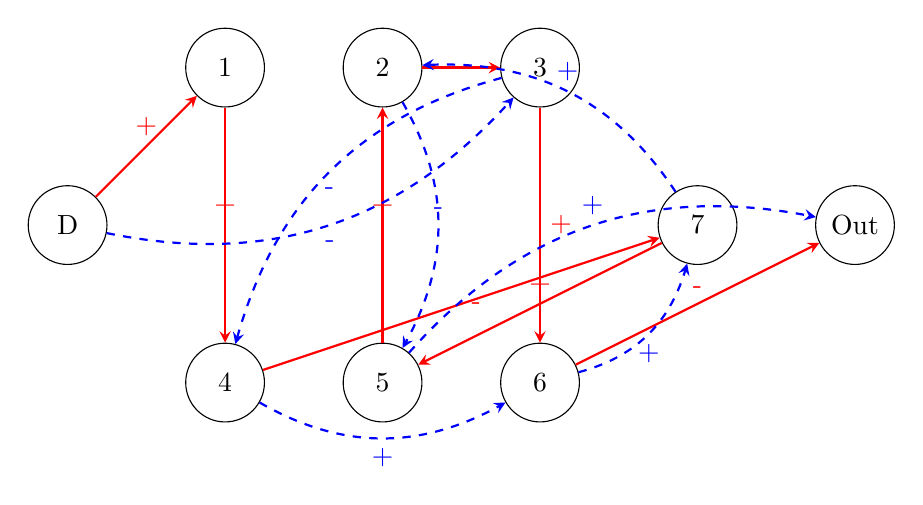
\begin{tikzpicture}[
        state/.style={circle,draw,minimum size=1cm},
        transition/.style={->,>=stealth,thick}
    ]
        % States
        \node[state] (D) at (0,0) {D};
        \node[state] (1) at (2,2) {1};
        \node[state] (2) at (4,2) {2};
        \node[state] (3) at (6,2) {3};
        \node[state] (4) at (2,-2) {4};
        \node[state] (5) at (4,-2) {5};
        \node[state] (6) at (6,-2) {6};
        \node[state] (7) at (8,0) {7};
        \node[state] (8) at (10,0) {Out};
        
        % Red path transitions
        \draw[transition,red] (D) to node[above] {+} (1);
        \draw[transition,red] (1) to node[above] {+} (4);
        \draw[transition,red] (4) to node[right] {-} (7);
        \draw[transition,red] (7) to node[above] {+} (5);
        \draw[transition,red] (5) to node[above] {+} (2);
        \draw[transition,red] (2) to node[right] {-} (3);
        \draw[transition,red] (3) to node[right] {+} (6);
        \draw[transition,red] (6) to node[above] {-} (8);
        
        % Blue path transitions (dashed)
        \draw[transition,blue,dashed] (D) to[bend right] node[below] {-} (3);
        \draw[transition,blue,dashed] (3) to[bend right] node[below] {-} (4);
        \draw[transition,blue,dashed] (4) to[bend right] node[below] {+} (6);
        \draw[transition,blue,dashed] (6) to[bend right] node[below] {+} (7);
        \draw[transition,blue,dashed] (7) to[bend right] node[above] {+} (2);
        \draw[transition,blue,dashed] (2) to[bend left] node[above] {-} (5);
        \draw[transition,blue,dashed] (5) to[bend left] node[above] {+} (8);
    \end{tikzpicture}
    \caption{Nash Cipher State Machine Diagram}
    \label{fig:state-machine}
\end{figure}


\section{Security Analysis}
\subsection{Computational Security}
Nash's exponential conjecture states that for sufficiently complex enciphering systems, the computational work required to break them grows exponentially with key length...

\section{Hardware Implementation}
\subsection{Resource Requirements}
\begin{itemize}
    \item State machine logic
    \item Memory elements
    \item Permutation path routing
\end{itemize}

\end{document}